\subsection{De-drift Stabilizes Sizing and Gating}
\label{sec:eval-dedrift}

We first verify drift-invariance of the de-drifted statistic, then evaluate the scaling of sizing accuracy and the reliability region of three-state gating.

\paragraph{Stability under drift}
We sweep $q$ over ${0.2, 0.5, 0.9}$ and compare the
de-drifted energy against two controls: \texttt{raw\_sq\_sum}
($\sum_j \Delta_j^2$, raw second moment, no mean removal) and
\texttt{abs\_net\_sum} ($|\sum_j \Delta_j|$, first-order absolute moment).
Table~\ref{tab:c2-unified} reports all three statistics without bias correction.

For sizing, \texttt{raw\_sq\_sum} produces overestimation above
$10^4\%$ under strong drift (Table~\ref{tab:c2-unified}),
whereas de-drifted energy keeps the error within about 10\%;
with Bessel correction this narrows further to about 3\%
(Table~\ref{tab:c3-anchor}; Supplement~Table~\ref{tab:c2-3}).

For gating, $K_{\mathrm{eff}}/L$ computed from de-drifted energy
remains nearly invariant across drift levels
(${\sim}0.015$--$0.017$). In contrast, \texttt{abs\_net\_sum} gives similarly low values under
asymmetric drift ($q \neq 0.5$) but jumps to $0.425$ at $q{=}0.5$
(Table~\ref{tab:c2-unified}). At that point the concentrated
fault is misread as diffuse (cross-configuration robustness
in Supplement~\ref{sec:appendix-dedrift}).

\begin{table}[!thbp]
\caption{Sizing and gating stability under drift. Top: sizing \texttt{rel\_err}; bottom: gating $K_{\mathrm{eff}}/L$ (\texttt{heavy\_share}).}
\label{tab:c2-unified}
\centering
\small
\setlength{\tabcolsep}{3pt}

\begin{tabular}{@{}lclrr@{}}
\toprule
\textbf{Sizing (\texttt{rel\_err})} & $q$ & workload & median & p90 \\
\midrule
\texttt{raw\_sq\_sum}        & 0.2 & bimodal & \textbf{+16\,659\%} & \textbf{17\,418\%} \\
\texttt{raw\_sq\_sum}        & 0.9 & bimodal & \textbf{+29\,576\%} & \textbf{31\,180\%} \\
\texttt{dedrift\_countscore} & 0.2 & bimodal & $-$9.1\%   & -4.1\% \\
\texttt{dedrift\_countscore} & 0.9 & bimodal & $-$8.9\%   & -3.7\% \\
\midrule
\textbf{Gating} ($K_{\mathrm{eff}}/L$) & $q$ & & \multicolumn{2}{c}{$K_{\mathrm{eff}}/L$} \\
\midrule
\texttt{dedrift\_countscore} & 0.2 & & \multicolumn{2}{c}{0.0153} \\
\texttt{dedrift\_countscore} & 0.5 & & \multicolumn{2}{c}{0.0166} \\
\texttt{dedrift\_countscore} & 0.9 & & \multicolumn{2}{c}{0.0162} \\
\texttt{abs\_net\_sum}       & 0.5 & & \multicolumn{2}{c}{\textbf{0.425}} \\
\bottomrule
\end{tabular}
\end{table}

\paragraph{Predictable scaling of sizing accuracy}
%\noindent\textbf{Predictable scaling of sizing accuracy} \quad
Multi-view fusion reduces $\mathrm{Std(rel\_err)}$ approximately as $V^{-0.5}$, consistent with the expected variance reduction from averaging near-independent views. A log-log regression across configurations yields a mean slope of $-0.498$ (std $0.050$), confirming this $V^{-0.5}$ scaling.
Increasing $m_0$ also reduces variance, as shown in Table~\ref{tab:c3-anchor}.

Moreover, $\mathrm{Std(rel\_err)}$ is weakly dependent on the discrepancy size~$D$: as it spans from $10^2$ to
$10^7$, the standard deviation remains in the approximately 2\%--3\% range, indicating that accuracy is governed primarily by probe capacity parameters rather than discrepancy magnitude (theoretical analysis, full curves, and stability verification in Supplement~\ref{sec:appendix-sizing-supp}).

\begin{table}[!htbp]
\caption{Representative configurations for sizing accuracy ($L{=}2048$). Top: fixing $m_0{=}32$ and sweeping $V$; bottom: fixing $V{=}4$ and sweeping $m_0$.}
\label{tab:c3-anchor}
\centering
\footnotesize
\begin{tabular}{lccc}
\toprule
Setting & Knob & Values & \texttt{Std(rel\_err)} (\%) \\
\midrule
\shortstack[l]{$m_0{=}32$} & $V$ & 1 / 4 / 16 & 3.53 / 2.25 / 1.01 \\
\shortstack[l]{$V{=}4$} & $m_0$ & 8 / 32 / 128 & 3.81 / 2.25 / 1.04 \\
\bottomrule
\end{tabular}
\end{table}

\paragraph{Three-state gating classification}
%\noindent\textbf{Three-state gating classification} \quad
The scale separation between concentrated and diffuse regimes
predicted in \S\ref{sec:gating} requires sufficient occupancy;
we now evaluate the practical reliability region of this
separation using the FAR--FRR trade-off over all samples
(including \texttt{unknown}).



Figure~\ref{fig:dedrift-far-frr-all} shows the unconditional
FAR--FRR Pareto front: each curve corresponds to a fixed
$\tau_{\text{occ}}$, and moving along a curve sweeps
$\tau_{\text{gating}}$.
Higher $\tau_{\text{occ}}$ generally yields lower FAR but
higher FRR. Raising the occupancy threshold excludes
ambiguous samples, improving discrimination among the
remainder and thus lowering FAR. However, because excluded
samples are counted as \texttt{unknown} rejections in the
unconditional metric, FRR rises accordingly.

Beyond $\tau_{\text{occ}} \approx 0.10$, the FRR floor settles
near 13\%. Two factors contribute: some genuinely diffuse
samples have occupancy below the threshold and are therefore
excluded as \texttt{unknown}; meanwhile, at large~$B$
(e.g., $B{=}200$, $L{=}2048$), the concentrated and diffuse
regimes converge in $K_{\text{eff}}/L$, making them
difficult to distinguish regardless of the threshold choice.

\begin{figure}[!htbp]
\centering
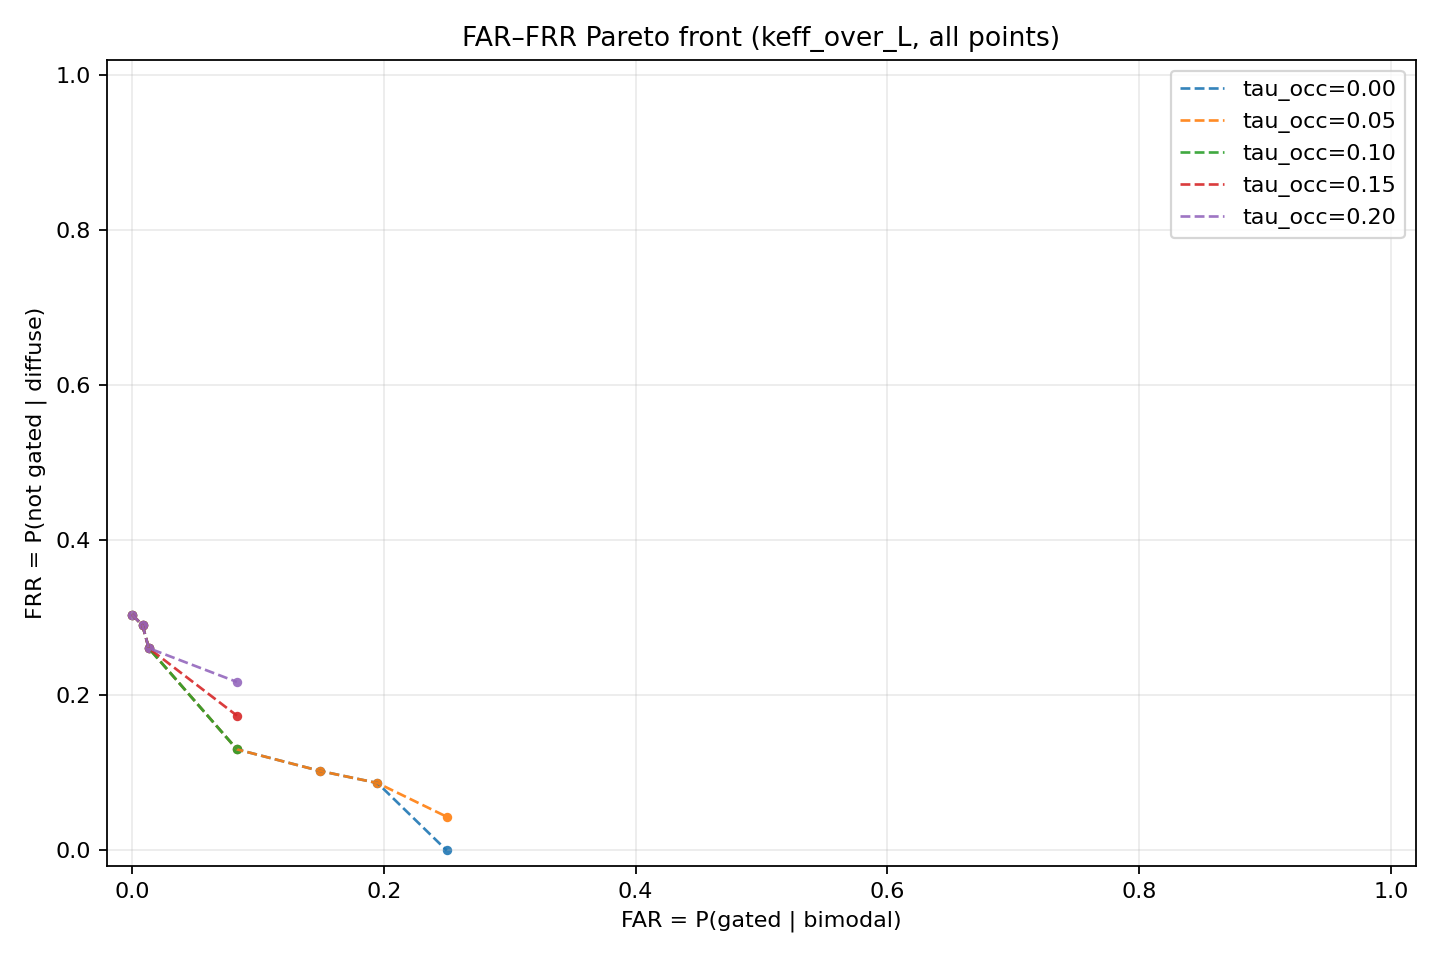
\includegraphics[width=0.95\linewidth]{figures/fig_far_frr_all_pareto.png}
\caption{Unconditional FAR--FRR trade-off. Each curve corresponds to a fixed $\tau_{\text{occ}}$; only non-dominated points are retained. Higher $\tau_{\text{occ}}$ generally yields lower FAR but higher FRR.}
\label{fig:dedrift-far-frr-all}
\end{figure}

The preceding analysis counts all samples---including those
labeled \texttt{unknown}---toward the error rates. An
alternative view considers only samples that receive a
decisive verdict (\texttt{notgate} or \texttt{gate}) and
computes \emph{conditional} error rates
$\mathrm{FAR_{cond}}$ and $\mathrm{FRR_{cond}}$ on this
subset. Under this metric, both rates can approach 0
simultaneously (Supplement Fig.~\ref{fig:dedrift-far-frr-cond}).
At $\tau_{\text{occ}}{=}0.10$, approximately 87\% of diffuse
samples still receive a decisive classification, while most
bimodal samples with small~$B$ are labeled \texttt{unknown}
due to low occupancy.
A two-state classifier would be forced to emit a verdict on
these low-support samples despite collapsed scale separation,
whereas the three-state design abstains and keeps
$\mathrm{FAR_{cond}}$ and $\mathrm{FRR_{cond}}$ near zero
among decisive verdicts.
